% This file is iccc.tex.  It contains the formatting instructions for and acts as a template for submissions to ICCC.  It borrows liberally from the AAAI and IJCAI formats and instructions.  It uses the files iccc.sty, iccc.bst and iccc.bib, the first two of which also borrow liberally from the same sources.

\documentclass[letterpaper]{article}
\usepackage{iccc}
\usepackage{times}
\usepackage{helvet}
\usepackage{courier}
\usepackage{graphicx}
\usepackage{caption}
\usepackage{subcaption}
\usepackage{amsmath}
\usepackage{amssymb}
\usepackage{booktabs}
\usepackage{algorithmic}
\usepackage{algorithm}

\graphicspath{ {images/} }

\newcommand\mydots{\hbox to .75em{.\hss.\hss.}}

\pdfinfo{
/Title (Chorus Identification in Lyrical, Sectional-Form Symbolic Music)
%/Subject (Proceedings of ICCC)
/Author (Anonymized)}
%/Author (Paul Bodily)}
% The file iccc.sty is the style file for ICCC proceedings.
%
\title{Chorus Identification in Lyrical, Sectional-Form Symbolic Music}
%\author{Paul Bodily, and Dan Ventura\\
%Computer Science Department\\
%Brigham Young University\\
%Provo, UT 84602  USA\\
%paulmbodily@gmail.com, ventura@cs.byu.edu\\
%}
\author{\emph{Anonymized}\\
\\
\\
\\
\\}
\setcounter{secnumdepth}{0}

\begin{document} 
\maketitle
\begin{abstract}
\begin{quote}
The identification of chorus segments in sectional-form music is essential to analyzing verse-chorus segmentation in symbolic music composition. This is a fundamentally different problem than detecting choruses in audio signals with important implications for being able to analyze and compare music on a structural, symbolic level. We define the chorus-identification problem. We describe the application of sequence alignment methods and deep learning methods to solving this problem. We report accuracies of each method on a dataset of pop leadsheets. We discuss the limitations of using the chorus-identification problem for characterizing high-level structure in pop music generally.
\end{quote}
\end{abstract}

\section{Introduction}

\section{Methods}
We present two general approaches to solving the chorus-identification problem: sequence alignment using a genetic algorithm to determine hyperparameters; and a bidirectional long short-term memory (LSTM) model.

\subsection{Sequence Alignment}

\subsection{Bidirectional LSTM}

\section{Results}

\begin{figure*}[th]
    \centering
    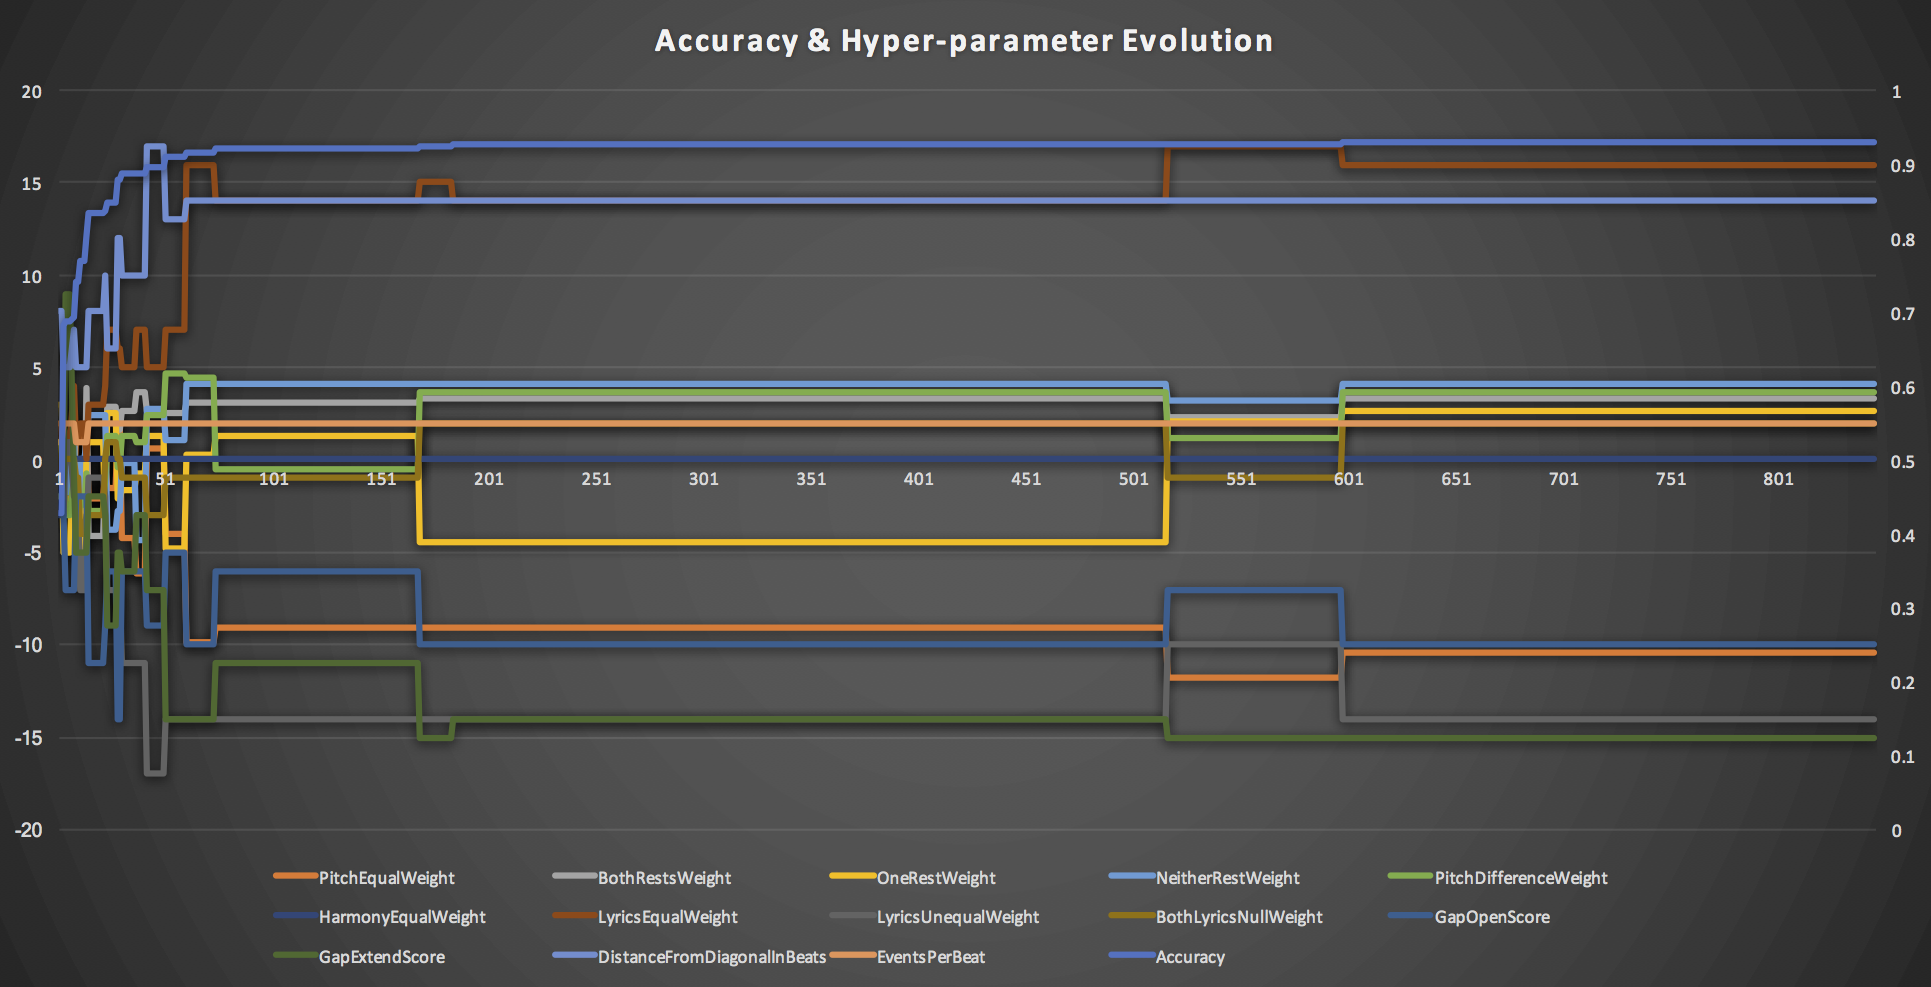
\includegraphics[width=\textwidth]{graph}
    \caption{This shows the accuracy increasing over generations for each of the different feature-set runs. Use arrows and labels to show what is learned at each big jump in accuracy. It also is showing how each of the (interesting) parameters fluctuates over time.}
    \label{fig:smallmultiple}
\end{figure*}

\begin{figure*}[th]
    \centering
    \begin{subfigure}{.2\textwidth}
        \includegraphics[width=\linewidth]{firstsmallmultiple}
        \caption{\emph{[INSERT HYPERPARAMS]\\hi}}
    \end{subfigure}
   % \\~\\ %add desired spacing between images, e. g. ~, \quad, \qquad, \hfill etc. 
    %(or a blank line to force the subfigure onto a new line)
   \begin{subfigure}{.2\textwidth}
        \includegraphics[width=\linewidth]{secondsmallmultiple}
        \caption{\emph{[INSERT HYPERPARAMS2]\\hi}}
    \end{subfigure}
    \begin{subfigure}{.2\textwidth}
        \includegraphics[width=\linewidth]{firstsmallmultiple}
        \caption{\emph{[INSERT HYPERPARAMS]\\hi}}
    \end{subfigure}
   % \\~\\ %add desired spacing between images, e. g. ~, \quad, \qquad, \hfill etc. 
    %(or a blank line to force the subfigure onto a new line)
   \begin{subfigure}{.2\textwidth}
        \includegraphics[width=\linewidth]{secondsmallmultiple}
        \caption{\emph{[INSERT HYPERPARAMS2]\\hi}}
    \end{subfigure}
    \caption{\emph{Using Genetic Algorithms to Determine Hyperparameters}. }\label{fig:smallmultiple}
\end{figure*}

\begin{table}[]
\centering
\caption{Time and accuracy for each run with bold for best}
\label{my-label}
\begin{tabular}{lllll}
 &  &  &  &  \\
 &  &  &  &  \\
 &  &  &  &  \\
 &  &  &  & 
\end{tabular}
\end{table}

\section{Discussion}

Here we talk about how many sectional-form songs don't have traditional choruses, but rather have sections where different viewpoints may or may not repeat. Like Hey Jude or even songs with multiple choruses like Don't stop believing.

Our next venture is to consider how to adapt these models for the chorus-identification problem to be able to recognize high-level repetitive structure across arbitrary viewpoints and to use these models to generate new songs from existing architectures. Of course the next step is then to figure out how to create novel architectures either \emph{de novo} or by intelligently combining existing architectures.

That's what makes choruses special, all the voiewpoints are repeating

Can we score structures?

\section{Conclusion}
viewpoint-centric self-similarity


\bibliographystyle{iccc}
\bibliography{bib}

\end{document}